

Observacion: \textcolor{red}{(enumerar)}.Si en la definicion \textcolor{red}{(recuerdo de mate 1. poner referencia)} cambiemos  $A \subset \mathbb{R}$ y $B \subset \mathbb{R}$ por $A \subset \mathbb{R}^{n}$ y $B \subset \mathbb{R}^{m}$  obtenemos de manera analoga la siguiente definici\'on.    



\begin{definition} Un campo $\mathbf{F}$ es una funci\'on  tal que
    $\mathbf{F}:A\subseteq \mathbb{R}^n \rightarrow B \subseteq \mathbb{R}^m.$   Si $m=1$ lo llamaremos  \textit{ campo vectorial }  y  si  $m\geq 2$ lo llamaremos   \textit{ campo escalar}. Al igual que en  \textcolor{red}{(recuerdo de mate 1. poner referencia)} a los conjuntos $A$ y $B$  se los llama, respectivamente, \textit{dominio}  y \textit{codominio} del campo $F$ y  la notaci\'on usual para los mismos  es  $A=\text{Dom}( \mathbf{F})$ y $B=\text{Cod}( \mathbf{F})$.   
  \end{definition}
  
  
  
  Notaci\'on:  \textcolor{red}{(enumerar)}  En general,  para nombrar a   campos escalars lo haremos con  letras minúsculas de imprenta y para nombrar a   campos vectorials lo haremos con  letras mayúsculas de imprenta.
  
  \begin{definition}
  Sea   $\mathbf{F}:A\subseteq \mathbb{R}^n \rightarrow B \subseteq \mathbb{R}^m$   un campo vectorial, dado $\boldsymbol{X} \in A$ se puede pensar a  $\mathbf{F}(\boldsymbol{X})$   como la evaluación de $m$ campos escalares en $\boldsymbol{X}$, 
    es decir,
    \begin{equation*}
        \mathbf{F}(\boldsymbol{X})=(f_0(\boldsymbol{X}), f_1(\boldsymbol{X}),..., f_m(\boldsymbol{X})).
    \end{equation*}
  Para $1 \leq i \leq n$,  el campo escalar $f_i: A\subseteq \mathbb{R}^n \rightarrow  \mathbb{R}$ se llama la \textit{i-\'esima componente} de $\mathbf{F}.$
 \end{definition}
  
  
  \begin{definition}
    Sea  $\mathbf{F}:A\subseteq \mathbb{R}^n \rightarrow B \subseteq \mathbb{R}^m$, se define el conjunto im\'agen de $\mathbf{F}$, y se nota $ \text{Img}(\mathbf{F})$, a 
    \begin{equation*}
        \text{Img}(\mathbf{F})=\{\boldsymbol{Y}\in\mathbb{R}^m: \mathbf{F}(\boldsymbol{X})=\boldsymbol{Y}, \boldsymbol{X} \in A\}
    \end{equation*}
  \end{definition}
  
  
    \begin{example}  \label{ej:campoVectorial}
        La función $\boldsymbol{T}:\mathbb{R}^2 \rightarrow \mathbb{R}^3 / \boldsymbol{T}(x,y) = (x+y,x-y,xy)$
        es un campo vectorial. 
       
        \textcolor{red}{decir quies es dominio, imagen, las componentes, y hacer un dibujo del dominio al codominio y sus componentes, revisar que todo lo pedido este definido previamente }
       
        \begin{equation*}
            \boldsymbol{T}(1,1)=(2,0,1)
        \end{equation*}
      
    \end{example}






\begin{example}
        La función $d:\mathbb{R}^3 \rightarrow \mathbb{R} / d(x,y,z) = \sqrt{x^2+y^2+z^2}$
        es un campo escalar.  
    \end{example} 
   
     \textcolor{red}{decir quies es dominio, imagen, las componentes, y hacer un dibujo del dominio al codominio }      
        
       Observacion: \textcolor{red}{ENUMERAR} En particular, si se piensa el vector argumento como un punto en el espacio, $d$ devuelve su distancia euclidea al orígen.
        \begin{equation*}
            \Rightarrow d(1,2,3)=\sqrt{1^2+2^2+3^2}=\sqrt{14}
        \end{equation*}
        \label{ej:campoEscalar}
  


    \begin{example}
    Probar que el campo $T(x,y) = (x+y,x-y,x+y)$  es una transformaci\'on lineal, es decir, que cumple  la condi\'on de   (\ref{tl}). Calcular su dominio, Imagen y mostrar sus componetes.
    
     \textcolor{red}{Resolver hacer un dibujo de dominio y codominio}
    
   \end{example}


\begin{definition} Se llaman parametrizaciones a las funciones de la forma $\boldsymbol{\sigma}:A\subseteq\mathbb{R}\rightarrow B\subseteq\mathbb{R}^m$ con $ m>1$.   
\end{definition}
   
   
   Notaci\'on:  \textcolor{red}{(enumerar)}  En general,  a una  parametrización se la suele notar con una letra min\'uscula del alfabeta griego.

    \begin{example} Hallar una parametrizacion del conjuto 
      \begin{equation*}
    C = \{  (x,y)  \in \mathbb{R}^2 \:|\:   x^2+y^2=r^2 \}.
    \end{equation*}  
        
        Para parametrizar una circunferencia, primero pensemos en el circulo unitario.
        En el circulo unitario, la abcisa (coordenada x) de cualquier punto es el coseno del ángulo que forma el eje horizontal con el segmento de radio
        que une el origen con tal punto. Asimismo, el seno del ángulo representa la ordenada (coordenada y).
        \begin{figure}[H] 
            \centering
            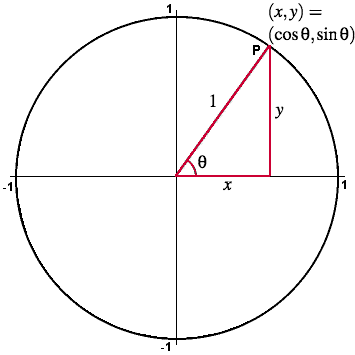
\includegraphics[width=0.5\textwidth]{../figs/unitCircle1.png} % Cambia esta ruta por la ubicación de tu imagen
            \caption{Coordenadas de los puntos sobre una circunferencia unitaria.}
            \label{fig:unitCircle1} % Etiqueta para hacer referencia a la imagen
        \end{figure}
        Por lo tanto, se propone una parametrización de la circunferencia unitaria de la forma:
        \begin{equation*}
            \boldsymbol{\sigma}:[0,2\pi)\rightarrow\mathbb{R}^2/ \\ \boldsymbol{\sigma}(t)=(\cos{t},\sin{t})
        \end{equation*}
        Así, si se graficase $\text{Img}(\boldsymbol{\sigma})$ como puntos en el plano se obtendría toda la circunferencia unitaria.
        Vale aclarar que se tomó el dominio como cerrado en $0$ y abierto en $2\pi$, para que, puesto que ambos valores de 
        entrada corresponden al mismo punto de salida, la parametrización no tenga "puntos repetidos", es decir, que sea inyectiva 
        (análogo a la inyectividad de funciones de $\mathbb{R}$ a $\mathbb{R}$).
        
         \end{example}
          \begin{example}    
        Hallar una parametrizaci\'on del conjuto 
          \begin{equation*}  
    C = \{  (x,y)  \in \mathbb{R}^2 \:|\:   (x-x_0)^2+(y-y_0)^2=r^2 \}
    \end{equation*} 
         Para contemplar circunferencias de radio distinto de $r$ centro $(0,0)$ vale con multiplicar por el radio a cada componente de la parametrización    \textcolor{red}{referencia}
        Además, para parametrizar aquellas que no estén centradas en el orígen, se desplaza cada punto de salida de la
        parametrización por $(x_0,y_0)$, el centro de la nueva circunferencia.
        Por lo tanto, la parametrización de una circunferencia de radio $r\in\mathbb{R}^+$ centrada en $(x_0,y_0)$ es:
        \begin{equation*}
            \boldsymbol{\sigma}:[0,2\pi)\rightarrow\mathbb{R}^2/ \\ \boldsymbol{\sigma}(t)=(r\cdot\cos{t}+x_0,r\cdot\sin{t}+y_0)
        \end{equation*} 
        
        \textcolor{red}{Agregar la otra manera de  parametrizacion de la circunferencia con el dibujo y la explicacion  }
        
    \end{example}
